\documentclass{standalone}
\usepackage{tikz}
\usetikzlibrary{patterns, positioning}


\begin{document}
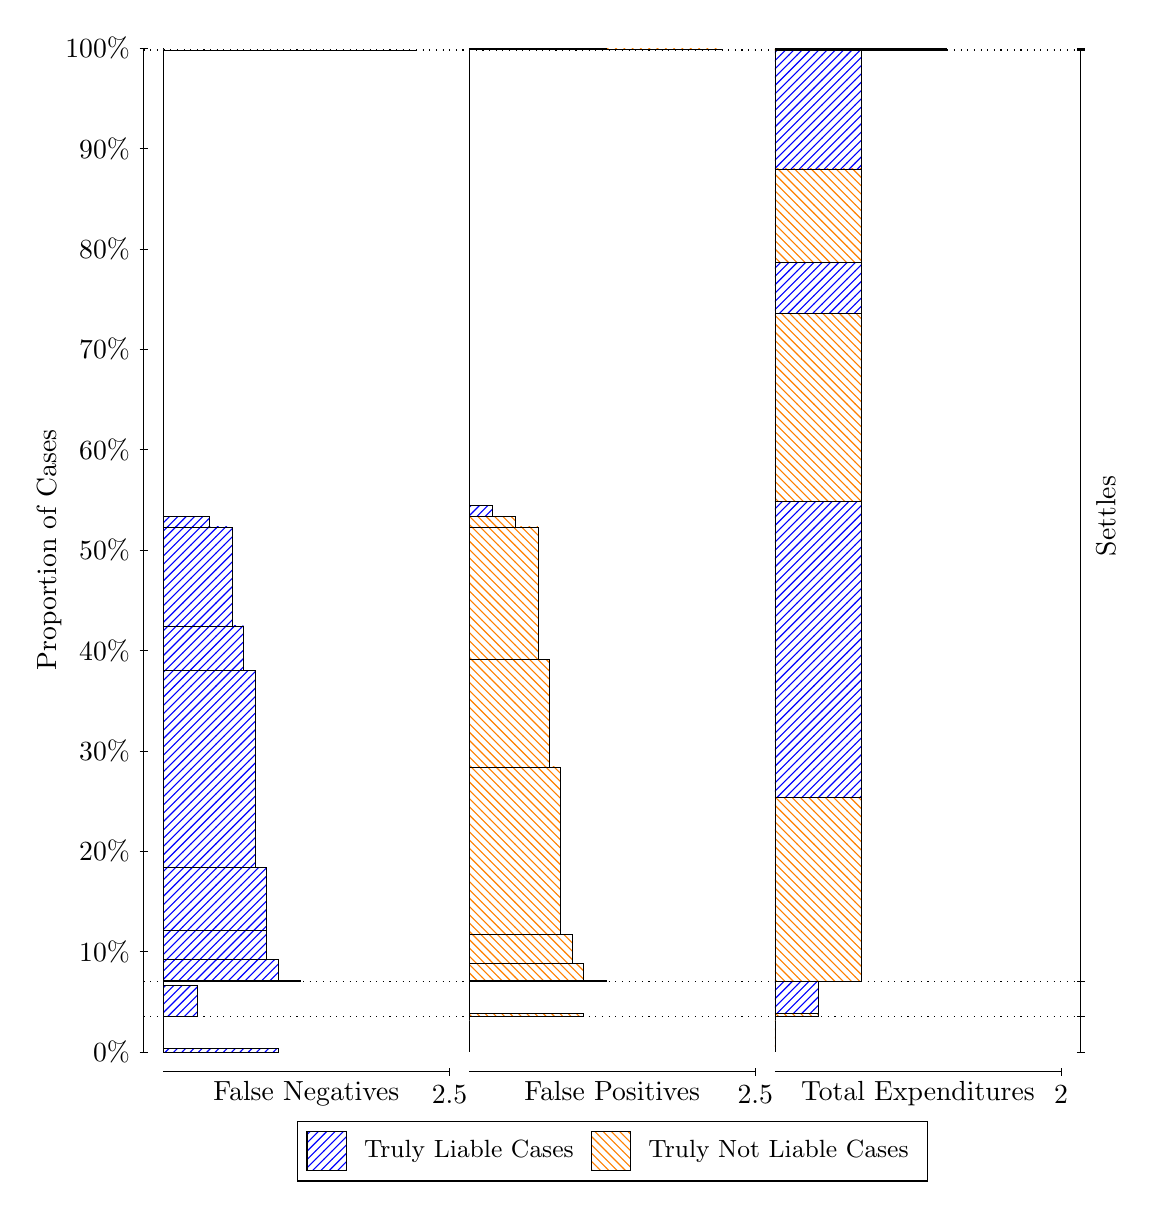
\begin{tikzpicture}
\draw[black, very thin] (1.5,1.75) -- (1.5,14.5);
\node[rotate=90, text=black, anchor=center] at (0.3, 8.125) {Proportion of Cases};
\draw[black, very thin] (1.45,1.75) -- (1.55,1.75);
\node[text=black, anchor=east] at (1.45, 1.75) {0\%};
\draw[black, very thin] (1.45,3.025) -- (1.55,3.025);
\node[text=black, anchor=east] at (1.45, 3.025) {10\%};
\draw[black, very thin] (1.45,4.3) -- (1.55,4.3);
\node[text=black, anchor=east] at (1.45, 4.3) {20\%};
\draw[black, very thin] (1.45,5.575) -- (1.55,5.575);
\node[text=black, anchor=east] at (1.45, 5.575) {30\%};
\draw[black, very thin] (1.45,6.85) -- (1.55,6.85);
\node[text=black, anchor=east] at (1.45, 6.85) {40\%};
\draw[black, very thin] (1.45,8.125) -- (1.55,8.125);
\node[text=black, anchor=east] at (1.45, 8.125) {50\%};
\draw[black, very thin] (1.45,9.4) -- (1.55,9.4);
\node[text=black, anchor=east] at (1.45, 9.4) {60\%};
\draw[black, very thin] (1.45,10.675) -- (1.55,10.675);
\node[text=black, anchor=east] at (1.45, 10.675) {70\%};
\draw[black, very thin] (1.45,11.95) -- (1.55,11.95);
\node[text=black, anchor=east] at (1.45, 11.95) {80\%};
\draw[black, very thin] (1.45,13.225) -- (1.55,13.225);
\node[text=black, anchor=east] at (1.45, 13.225) {90\%};
\draw[black, very thin] (1.45,14.5) -- (1.55,14.5);
\node[text=black, anchor=east] at (1.45, 14.5) {100\%};

\draw[black, very thin] (13.4,1.75) -- (13.4,14.5);
\draw[black, very thin] (13.35,1.75) -- (13.45,1.75);
\node[anchor=west] at (13.35, 1.75) {};
\draw[black, very thin] (13.35,2.1971) -- (13.45,2.1971);
\node[anchor=west] at (13.35, 2.1971) {};
\draw[black, very thin] (13.35,2.6443) -- (13.45,2.6443);
\node[anchor=west] at (13.35, 2.6443) {};
\draw[black, very thin] (13.35,14.466) -- (13.45,14.466);
\node[anchor=west] at (13.35, 14.466) {};
\draw[black, very thin] (13.35,14.483) -- (13.45,14.483);
\node[anchor=west] at (13.35, 14.483) {};
\draw[black, very thin] (13.35,14.5) -- (13.45,14.5);
\node[anchor=west] at (13.35, 14.5) {};

\draw[black, very thin, pattern color=blue, pattern=north east lines] (1.75,1.75) rectangle (3.2033,1.797);
\draw[black, very thin, pattern color=orange, pattern=north west lines] (1.75,1.797) rectangle (1.75,2.1971);
\draw[black, very thin, pattern color=blue, pattern=north east lines] (1.75,2.1971) rectangle (2.186,2.5973);
\draw[black, very thin, pattern color=orange, pattern=north west lines] (1.75,2.5973) rectangle (1.75,2.6443);
\draw[black, very thin, pattern color=blue, pattern=north east lines] (1.75,2.6443) rectangle (3.494,2.6623);
\draw[black, very thin, pattern color=blue, pattern=north east lines] (1.75,2.6623) rectangle (3.2033,2.9248);
\draw[black, very thin, pattern color=blue, pattern=north east lines] (1.75,2.9248) rectangle (3.058,3.2936);
\draw[black, very thin, pattern color=blue, pattern=north east lines] (1.75,3.2936) rectangle (3.058,4.0958);
\draw[black, very thin, pattern color=blue, pattern=north east lines] (1.75,4.0958) rectangle (2.9127,6.5959);
\draw[black, very thin, pattern color=blue, pattern=north east lines] (1.75,6.5959) rectangle (2.7673,7.1604);
\draw[black, very thin, pattern color=blue, pattern=north east lines] (1.75,7.1604) rectangle (2.622,8.4198);
\draw[black, very thin, pattern color=blue, pattern=north east lines] (1.75,8.4198) rectangle (2.3313,8.5552);
\draw[black, very thin, pattern color=orange, pattern=north west lines] (1.75,8.5552) rectangle (1.75,14.466);
\draw[black, very thin, pattern color=blue, pattern=north east lines] (1.75,14.466) rectangle (4.9473,14.472);
\draw[black, very thin, pattern color=orange, pattern=north west lines] (1.75,14.472) rectangle (1.75,14.483);
\draw[black, very thin, pattern color=orange, pattern=north west lines] (1.75,14.483) rectangle (1.75,14.489);
\draw[black, very thin, pattern color=blue, pattern=north east lines] (1.75,14.489) rectangle (1.75,14.5);
\draw[black, very thin, pattern color=orange, pattern=north west lines] (5.6333,1.75) rectangle (5.6333,2.1501);
\draw[black, very thin, pattern color=blue, pattern=north east lines] (5.6333,2.1501) rectangle (5.6333,2.1971);
\draw[black, very thin, pattern color=orange, pattern=north west lines] (5.6333,2.1971) rectangle (7.0867,2.2442);
\draw[black, very thin, pattern color=blue, pattern=north east lines] (5.6333,2.2442) rectangle (5.6333,2.6443);
\draw[black, very thin, pattern color=orange, pattern=north west lines] (5.6333,2.6443) rectangle (7.3773,2.6623);
\draw[black, very thin, pattern color=orange, pattern=north west lines] (5.6333,2.6623) rectangle (7.0867,2.8766);
\draw[black, very thin, pattern color=orange, pattern=north west lines] (5.6333,2.8766) rectangle (6.9413,3.2454);
\draw[black, very thin, pattern color=orange, pattern=north west lines] (5.6333,3.2454) rectangle (6.796,5.3708);
\draw[black, very thin, pattern color=orange, pattern=north west lines] (5.6333,5.3708) rectangle (6.6507,6.7376);
\draw[black, very thin, pattern color=orange, pattern=north west lines] (5.6333,6.7376) rectangle (6.5053,8.4199);
\draw[black, very thin, pattern color=orange, pattern=north west lines] (5.6333,8.4199) rectangle (6.2147,8.5555);
\draw[black, very thin, pattern color=blue, pattern=north east lines] (5.6333,8.5555) rectangle (5.924,8.6909);
\draw[black, very thin, pattern color=blue, pattern=north east lines] (5.6333,8.6909) rectangle (5.6333,14.466);
\draw[black, very thin, pattern color=orange, pattern=north west lines] (5.6333,14.466) rectangle (5.6333,14.477);
\draw[black, very thin, pattern color=blue, pattern=north east lines] (5.6333,14.477) rectangle (5.6333,14.483);
\draw[black, very thin, pattern color=orange, pattern=north west lines] (5.6333,14.483) rectangle (8.8307,14.489);
\draw[black, very thin, pattern color=blue, pattern=north east lines] (5.6333,14.489) rectangle (7.3773,14.5);
\draw[black, very thin, pattern color=orange, pattern=north west lines] (9.5167,1.75) rectangle (9.5167,2.1501);
\draw[black, very thin, pattern color=blue, pattern=north east lines] (9.5167,2.1501) rectangle (9.5167,2.1971);
\draw[black, very thin, pattern color=orange, pattern=north west lines] (9.5167,2.1971) rectangle (10.062,2.2442);
\draw[black, very thin, pattern color=blue, pattern=north east lines] (9.5167,2.2442) rectangle (10.062,2.6443);
\draw[black, very thin, pattern color=orange, pattern=north west lines] (9.5167,2.6443) rectangle (10.607,4.9841);
\draw[black, very thin, pattern color=blue, pattern=north east lines] (9.5167,4.9841) rectangle (10.607,8.7435);
\draw[black, very thin, pattern color=orange, pattern=north west lines] (9.5167,8.7435) rectangle (10.607,11.126);
\draw[black, very thin, pattern color=blue, pattern=north east lines] (9.5167,11.126) rectangle (10.607,11.775);
\draw[black, very thin, pattern color=orange, pattern=north west lines] (9.5167,11.775) rectangle (10.607,12.964);
\draw[black, very thin, pattern color=blue, pattern=north east lines] (9.5167,12.964) rectangle (10.607,14.466);
\draw[black, very thin, pattern color=orange, pattern=north west lines] (9.5167,14.466) rectangle (11.697,14.477);
\draw[black, very thin, pattern color=blue, pattern=north east lines] (9.5167,14.477) rectangle (11.697,14.483);
\draw[black, very thin, pattern color=orange, pattern=north west lines] (9.5167,14.483) rectangle (11.697,14.489);
\draw[black, very thin, pattern color=blue, pattern=north east lines] (9.5167,14.489) rectangle (11.697,14.5);
\draw[black, dotted] (1.5,2.1971) -- (13.4,2.1971);
\draw[black, dotted] (1.5,2.6443) -- (13.4,2.6443);
\draw[black, dotted] (1.5,14.466) -- (13.4,14.466);
\draw[black, dotted] (1.5,14.483) -- (13.4,14.483);
\draw[black, very thin] (1.75,1.5) -- (5.3833,1.5);
\node[text=black, anchor=north] at (3.5667, 1.5) {False Negatives};
\draw[black, very thin] (5.3833,1.45) -- (5.3833,1.55);
\node[text=black, anchor=north] at (5.3833, 1.45) {2.5};

\draw[black, very thin] (5.6333,1.5) -- (9.2667,1.5);
\node[text=black, anchor=north] at (7.45, 1.5) {False Positives};
\draw[black, very thin] (9.2667,1.45) -- (9.2667,1.55);
\node[text=black, anchor=north] at (9.2667, 1.45) {2.5};

\draw[black, very thin] (9.5167,1.5) -- (13.15,1.5);
\node[text=black, anchor=north] at (11.333, 1.5) {Total Expenditures};
\draw[black, very thin] (13.15,1.45) -- (13.15,1.55);
\node[text=black, anchor=north] at (13.15, 1.45) {2};



\node[text=black, centered, rotate=90] at (13.72, 8.5553) {Settles};



\draw (7.449999999999999,1.5) node[draw=none] (baseCoordinate) {};
\begin{scope}[align=center]
        \matrix[scale=0.5, draw=black, below=0.5cm of baseCoordinate, nodes={draw}, column sep=0.1cm]{
            \node[rectangle, draw, minimum width=0.5cm, minimum height=0.5cm, pattern color=blue, pattern=north east lines] {}; &
            \node[draw=none, font=\small, text=black] (B) {Truly Liable Cases}; &
            \node[rectangle, draw, minimum width=0.5cm, minimum height=0.5cm, pattern color=orange, pattern=north west lines] {}; &
            \node[draw=none, font=\small, text=black] (B) {Truly Not Liable Cases}; \\
            };
\end{scope}

\end{tikzpicture}
\end{document}